\documentclass[compress]{beamer}
\usepackage{ifthen,verbatim}

\title{Status of Muon Alignment II}
\author{Jim Pivarski, Alexei Safonov, K\'aroly Banicz$^*$}
\institute{Texas A\&M University, $^*$FermiLab}
\date{17 March, 2008}

\newcommand{\isnote}{}
\xdefinecolor{lightyellow}{rgb}{1.,1.,0.25}
\xdefinecolor{darkblue}{rgb}{0.1,0.1,0.7}

%% Uncomment this to get annotations
%% \def\notes{\addtocounter{page}{-1}
%%            \renewcommand{\isnote}{*}
%% 	   \beamertemplateshadingbackground{lightyellow}{white}
%%            \begin{frame}
%%            \frametitle{Notes for the previous page (page \insertpagenumber)}
%%            \itemize}
%% \def\endnotes{\enditemize
%% 	      \end{frame}
%%               \beamertemplateshadingbackground{white}{white}
%%               \renewcommand{\isnote}{}}

%% Uncomment this to not get annotations
\def\notes{\comment}
\def\endnotes{\endcomment}

\setbeamertemplate{navigation symbols}{}
\setbeamertemplate{headline}{\mbox{ } \hfill
\begin{minipage}{5.5 cm}
\vspace{-0.75 cm} \small
\end{minipage} \hfill
\begin{minipage}{4.5 cm}
\vspace{-0.75 cm} \small
\begin{flushright}
\ifthenelse{\equal{\insertpagenumber}{1}}{}{Jim Pivarski \hspace{0.2 cm} \insertpagenumber\isnote/\pageref{numpages}}
\end{flushright}
\end{minipage}\mbox{\hspace{0.2 cm}}\includegraphics[height=1 cm]{../cmslogo} \hspace{0.1 cm} \includegraphics[height=1 cm]{../tamulogo} \hspace{0.01 cm} \vspace{-1.05 cm}}

\begin{document}
\frame{\titlepage}

%% \begin{notes}
%% \item This is the annotated version of my talk.
%% \item If you want the version that I am presenting, download the one
%% labeled ``slides'' on Indico (or just ignore these yellow pages).
%% \item The annotated version is provided for extra detail and a written
%% record of comments that I intend to make orally.
%% \item Yellow notes refer to the content on the {\it previous} page.
%% \item All other slides are identical for the two versions.
%% \end{notes}

% How we see subdivision of tasks
% Texas A&M, Karoly (FermiLab)
% track-based alignment with HIP procedure:
%     whole muon system, endcap and barrel
%     develop (DPG) and determine performance (POG) of
%         full-scale procedure
%         start-up procedures (Karoly for beam-halo)
%         tests with CRAFT (CRA0T?)
%     CSC layer alignment with tracks
%     apply procedures in data (beam-halo and first collisions)
%         to determine real chamber positions
%
% IFCA
% track-based alignment with MillePede procedure
%     whole muon system, endcap and barrel
%     DT layer and superlayer alignment
%
% Hardware alignment groups (IFCA, Florida, FermiLab, Wisconsin)
%     independent alignment of chambers and layers

\begin{frame}
\frametitle{How we see subdivision of tasks}

\vfill
\mbox{\hspace{-0.9 cm} 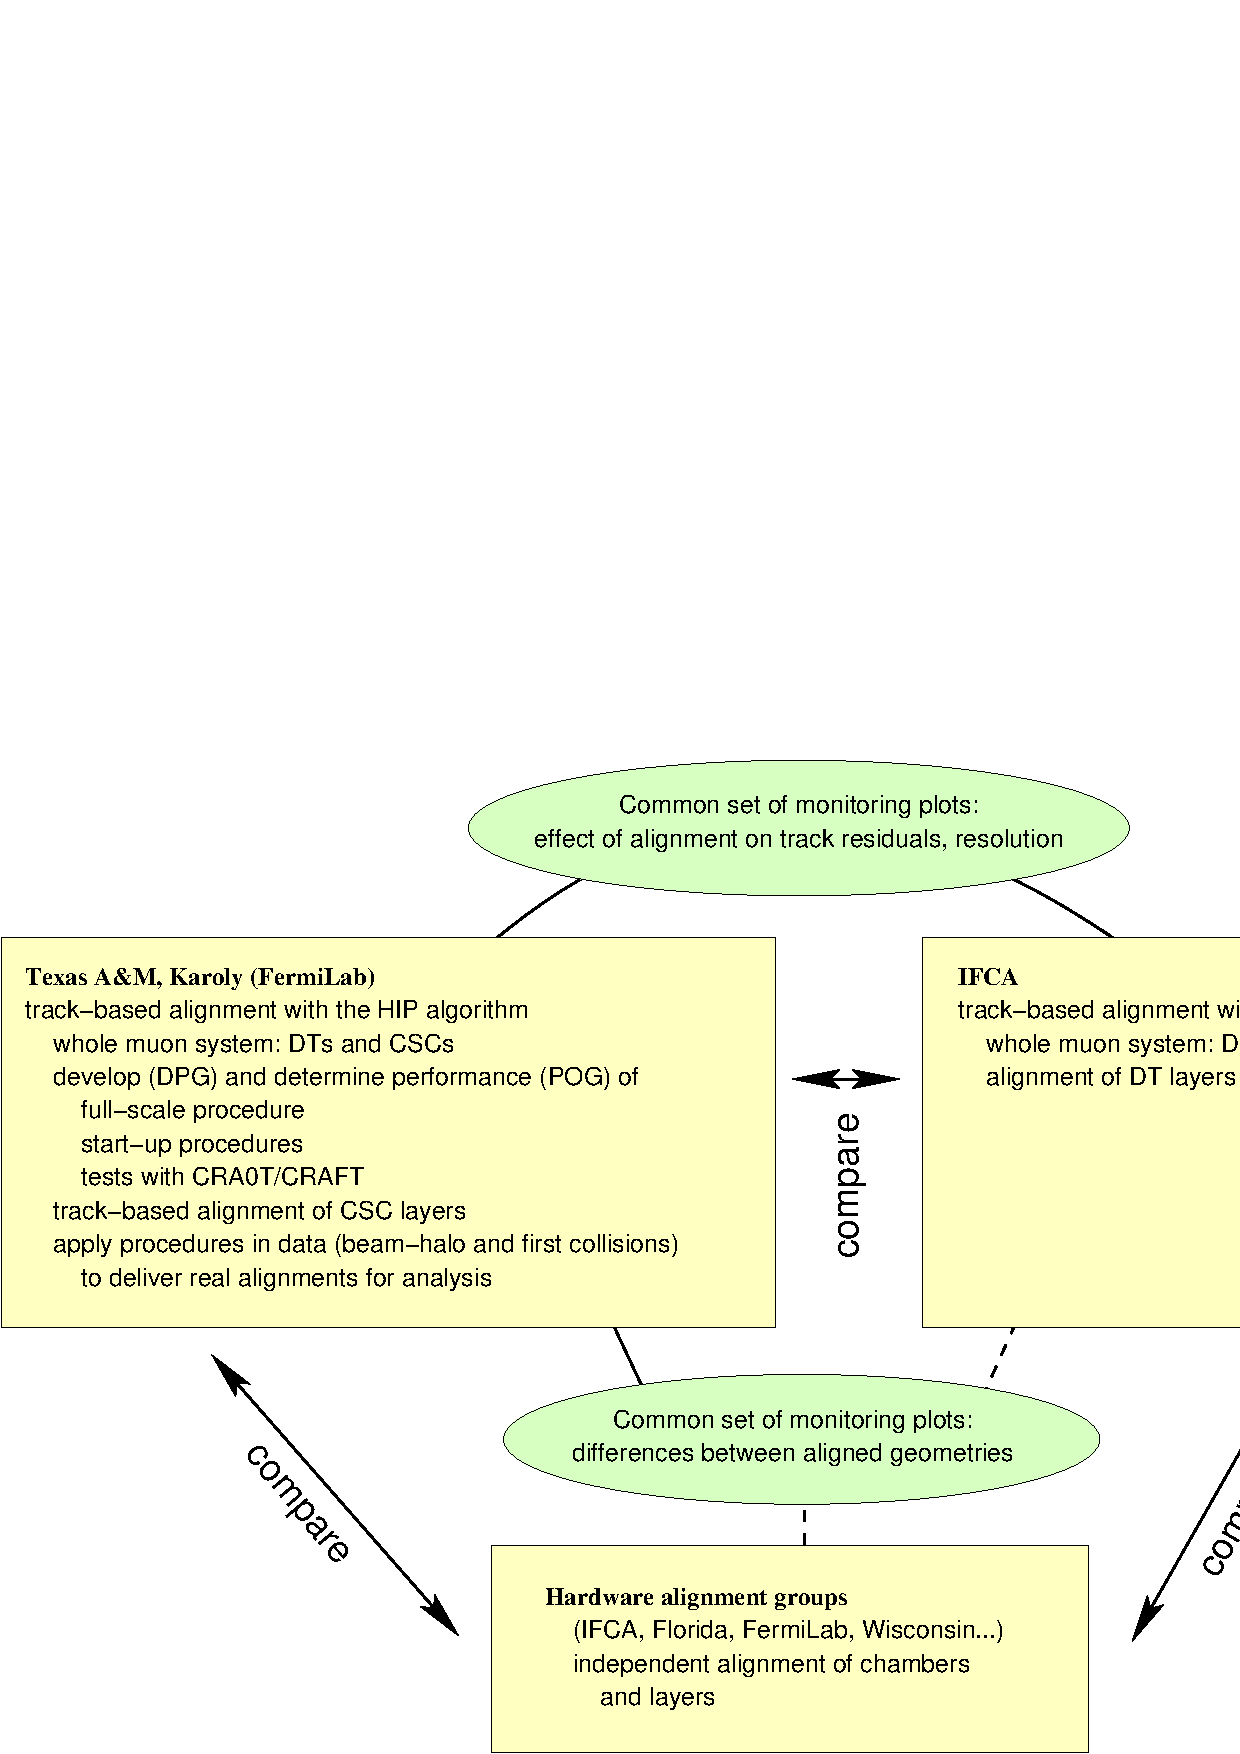
\includegraphics[width=1.15\linewidth]{groups.pdf}}
\end{frame}

% Status at a glance
% * software development:
%   * HIP is done and stable, MillePede is being ported to common framework
%   * Monitoring plots in progress
%     * On-board monitoring during alignment: done and in-use since last summer
%     * After-alignment validation with events: Javier is porting to DQM
%     * After-alignemnt comparison of geometries: infrastructure in place, but the plotter needs to be written
% * procedure development (tuning parameters, improving performance)
%   * current state: mm level
%   * a new cut has been shown to improve this dramatically ($\to$ hundreds of $\mu$m), but it hasn't been
%     fully integrated into the procedure; that's a project for the next month
%   * this can be studied with existing MC after we back-port software into 1_6_X
% * estimation of performance
%   * full study with systematic uncertainties has been performed before improvements, we can repeat it
%   * followed through to Z' studies in analysis note 2007/038 (some limited public results)
% * startup plans and comparison with hardware alignment
%   * developed detailed plans for how to analyze CRAFT, beam-halo, and first data
%   * plan includes points of contact with hardware alignment
%   * made sure all software needed for them is in 2_0_X, including trigger paths for special events (beam-halo)
% This talk will focus on the startup plans

\begin{frame}
\frametitle{Status at a glance}
\scriptsize

\begin{minipage}{\linewidth}
\textcolor{darkblue}{Software development (C++ and algorithms):}
\begin{itemize}
\item \scriptsize HIP is done and stable, MillePede is being ported to common framework
\item \scriptsize Monitoring plots in progress
\begin{itemize}
\item \scriptsize On-board monitoring during alignment iterations: done
\item \scriptsize After-alignment validation with events: Javier is porting to DQM
\item \scriptsize After-alignment comparison of geometries: infrastructure in place, but plots need to be defined
\end{itemize}
\end{itemize}

\textcolor{darkblue}{Procedure development (tuning parameters, improving performance):}
\begin{itemize}
\item \scriptsize Current state of HIP: mm level alignment of chambers relative to tracker
\item \scriptsize New track cut has been shown to improve this dramatically ($\to$ 100's of $\mu$m)
\item \scriptsize Needs to be fully incorporated, tested
\item \scriptsize Studies can begin now in 1\_6\_7 with existing MC
\end{itemize}

\textcolor{darkblue}{Estimation of alignment performance:}
\begin{itemize}
\item \scriptsize Performed full study, including systematic uncertainties, before improvements
\begin{itemize}
\item \scriptsize We can repeat it with updated procedure
\end{itemize}
\item \scriptsize Old study followed through to $Z'$ resolution in Analysis Note 2007/038
\end{itemize}
\end{minipage}

\textcolor{blue}{\fbox{\begin{minipage}{\linewidth}
\textcolor{darkblue}{Start-up plans:}
\begin{itemize}
\item \scriptsize Developed detailed plans for analyzing CRAFT, beam-halo, and first collisions
\item \scriptsize Plan includes points of contact with hardware alignment
\item \scriptsize Made sure all software in 2\_0\_X, including trigger paths for special data streams
\end{itemize}
\end{minipage}}}
\end{frame}

% startup plans

\begin{frame}
\frametitle{HIP-based alignment procedures}
\textcolor{darkblue}{1. Full-scale alignment of chambers to tracker (10 and 100~pb$^{-1}$, \\ \hfill not startup)}
\begin{itemize}
\item \textcolor{darkblue}{Basic idea:} tracker provides good tracks, we move
muon chambers to minimize ``track-minus-hit'' residuals on average
\item Therefore alignment is automatically relative to tracker
\item Residuals distributions are wide due to multiple scattering
\begin{itemize}
\item Gain precision by re-fitting tracks with different hit weights
in tracker and in each muon station
\item We use muon Alignment Parameter Errors (APEs) to set these
hit weights: APEs have been behaving as expected since last summer
\end{itemize}
\end{itemize}

\vspace{0.25 cm}
\textcolor{red}{$\to$ test} with selected chambers in CRAFT (CRA0T?)

\vspace{0.25 cm}
\textcolor{red}{$\to$ measure} all chambers ``for real'' when 10--100~pb$^{-1}$ are available
\end{frame}

\begin{frame}
\frametitle{HIP-based alignment procedures}

\begin{columns}
\column{0.8\linewidth}
\textcolor{darkblue}{2. Relative alignment of CSCs (low energy tracks \\ \hfill and/or beam-halo)}
\begin{itemize}
\item Locally fit tracks that pass through CSC overlap regions (again,
by setting APEs)
\item Align CSC chambers relative to their neighbors
\end{itemize}

\column{0.2\linewidth}
\includegraphics[width=\linewidth]{overlap.png}
\end{columns}

\textcolor{red}{$\to$ test} with horizontal cosmics in MTCC

\vspace{0.25 cm}
\textcolor{red}{$\to$ measure} all applicable chambers ``for real'' when enough \\ \hfill beam-halo and/or QCD muons are available

\vfill
\textcolor{darkblue}{3. Relative alignment of CSC layers}
\begin{itemize}
\item Same method as above, not restricted to overlap regions
\end{itemize}
\end{frame}

\begin{frame}
\frametitle{HIP-based alignment procedures}
\textcolor{darkblue}{4. Alignment of large structures to tracker (first collisions)}
\begin{itemize}
\item Treat large structures (barrel wheels and endcap rings) as individual alignable objects
\item Compliments relative measurements in combined \mbox{start-up program \hspace{-1 cm}}
\item Very few tracks needed: 1000~muons (0.1~pb$^{-1}$) yields \mbox{400~$\mu$m \hspace{-0.5 cm}} global precision when chambers have 500~$\mu$m local precision
\end{itemize}

\vspace{-0.25 cm}
\begin{center}
\includegraphics[height=0.6\linewidth, angle=90]{vsinternal.pdf}
\end{center}

\vspace{-0.25 cm}
\textcolor{red}{$\to$ measure} in the first week or two of collisions
\end{frame}

\begin{frame}
\frametitle{Real-data test for full procedure}
\begin{center}
\includegraphics[width=0.7\linewidth]{craft.pdf}
\end{center}

\scriptsize
\begin{itemize}
\item Test full-scale procedure on top and bottom chambers in muon
barrel (1 million muons through tracker?), possibly as far as ME1/3 (10k muons?)

\item Alignment output would be ``real,'' usable for reconstruction,
but this is primarily a test of the procedure
\end{itemize}
\end{frame}

\begin{frame}
\frametitle{Real-data test for beam-halo}

\vfill
\begin{columns}
\column{0.6\linewidth}
\includegraphics[width=\linewidth]{beam-halo_schematic.png}
\column{0.4\linewidth}
\includegraphics[width=\linewidth]{mtcc_chambers.png}
\end{columns}

\begin{itemize}
\item Pre-collisions beam-halo muons are ideal for relative CSC
alignment; procedures will be developed with these in mind
\item We can test the procedure in MTCC as soon as we're ready
\end{itemize}

\vfill
\hspace{-0.83 cm} \textcolor{darkblue}{\Large Readiness for real beam-halo data}
\begin{itemize}
\item L1 trigger in progress
\item HLT paths and event streams are ready
\end{itemize}
\end{frame}

\begin{frame}
\frametitle{Comparisons with hardware}

Opportunities for comparison with hardware alignment available in
\begin{itemize}
\item MTCC relative alignment of CSCs: hardware alignment already
exists and compares favorably with photogrammetry

\item Chambers selected for CRA0T/CRAFT alignment

\item Relative alignment of CSCs during beam-halo period (June)

\item Position of large structures relative to tracker in the first weeks of collisions
\end{itemize}

How would we do that comparison?
\begin{itemize}
\item Database comparison tool applied to alignment output in SQLite files (under development)
\end{itemize}

\vfill
\hspace{-0.83 cm} \textcolor{darkblue}{\Large {\it Combining} track-based and hardware alignment data?}

After verifying a mutually-measured direction, for example
\begin{itemize}
\item beam-halo and SLM lasers both measure CSC $r\phi$
\item only SLM lasers measure CSC $z$: use it if $r\phi$ agrees
\end{itemize}
\end{frame}

% Timeline
% * March:
%   1. infrastructure for comparing (and maybe manually changing) muon geometry in database: done two days ago, needs to be documented/publicized
%   2. back-port last HIP-related software updates to 1_6_7 to develop procedure with existing MC samples
%   3. implement first draft of a HIP alignment procedure with CSC overlap hits and pass it to Karoly for development on beam-halo
%   * develop DQM alignment validation
% * April:
%   * optimize large-dataset procedure with new track cut
%   * possibly hybrid procedure with overlap hits in CSCs
%   * determine expected performance with 0~T and 3.8~T cosmic rays
%   * apply to CRA0T dataset if that would be interesting
%   * develop database monitoring plots
%   * determine expected performance of CSC overlap method with beam-halo
%     * apply ``beam-halo'' procedure to nearly horizontal MTCC muons
% * May:
%   * Do systematics studies on re-optimized procedure, startup procedures, cosmic ray tests
%   * Update expected effect of misalignment on muon tracks, physics quantities
%   * apply procedure to CRAFT dataset
%     * compare with hardware measurements
% * June:
%   * use beam-halo tracks to align endcap chambers, possibly layers
%     * compare and/or combine with hardware measurements
% * July:
%   * align large structures with first 1000 tracks
%   * combine measurements (beam-halo, CRAFT, first 1000 tracks, hardware measurements, etc.)
% * and beyond:
%   * apply full-scale procedure

\begin{frame}
\frametitle{Timeline \textcolor{darkblue}{\small (POG-related steps in blue)}}
\scriptsize

\textcolor{black}{March:}
\begin{enumerate}
\item \scriptsize Infrastructure for database comparison and manual update (done)
\item \scriptsize Back-port last HIP-related software updates to 1\_6\_7 to use existing MC samples
\item \scriptsize Implement first draft of CSC overlap-hit alignment procedure
\end{enumerate}

\textcolor{black}{April:}
\begin{itemize}
\item \scriptsize Optimize large-dataset procedure with new track cut
\item \scriptsize Determine expected performance with 0~T and 3.8~T cosmic rays
\item \scriptsize \textcolor{darkblue}{Apply to CRA0T dataset if 0~T case is interesting}
\item \scriptsize Develop database comparison plots
\item \scriptsize Study CSC overlap-hit procedure in beam-halo MC (Karoly)
\begin{itemize}
\item \scriptsize \textcolor{darkblue}{Apply to horizontal MTCC muons as a test}
\end{itemize}
\end{itemize}

\vspace{-0.25 cm}
\textcolor{black}{May:}
\begin{itemize}
\item \scriptsize \textcolor{darkblue}{Full systematics studies with all procedures}
\item \scriptsize \textcolor{darkblue}{Update physics studies}
\item \scriptsize \textcolor{darkblue}{Apply procedure to CRAFT dataset}
\begin{itemize}
\item \scriptsize Compare with hardware measurements, if available
\end{itemize}
\end{itemize}

\vspace{-0.25 cm}
\textcolor{black}{June:}
\begin{itemize}
\item \scriptsize \textcolor{darkblue}{Use beam-halo tracks to get a real alignment of endcap chambers/layers}
\begin{itemize}
\item \scriptsize Compare/combine with hardware measurements, if available/in agreement
\end{itemize}
\end{itemize}

\vspace{-0.25 cm}
\textcolor{black}{July:}
\begin{itemize}
\item \scriptsize \textcolor{darkblue}{Align large structures with first 1000 muons}
\item \scriptsize Combine measurements where applicable (beam-halo,
CRAFT, first 1000 muons, hardware measurements, etc\ldots)
\end{itemize}

\textcolor{black}{and beyond:}
\begin{itemize}
\item \scriptsize \textcolor{darkblue}{Apply full-scale procedure}
\end{itemize}
\end{frame}

% CSA08 alignment scenarios, with Z' plot

\begin{frame}
\frametitle{CSA08 alignment scenarios}
\begin{columns}
\column{0.6\linewidth}
\includegraphics[height=\linewidth, angle=90]{ZSSM_Align10-100_MassRes_color.pdf}
\column{0.4\linewidth}
\begin{center}
CSA07 \textcolor{red}{10} and \textcolor{blue}{100~pb$^{-1}$} scenarios
were generated under different assumptions, and effect on high dimuon
masses didn't scale as expected
\end{center}
\end{columns}

\vspace{-0.5 cm}
\begin{columns}
\column{0.4\linewidth}

\begin{center}
CSA08 \textcolor{red}{0}, \textcolor{blue}{10}, and
\textcolor{black}{100~pb$^{-1}$} scenarios do scale as expected for a
3.5~TeV (extreme) $Z'$
\end{center}

\vspace{-0.25 cm}
\scriptsize
\begin{itemize}
\item Also incorporate new information from hardware and track-based alignments
\item More detailed model of uncertainties
\end{itemize}

\column{0.6\linewidth}
\vspace{0.5 cm}
\includegraphics[height=\linewidth, angle=90]{newscenarios_zprimetest.pdf}
\end{columns}
\end{frame}

\begin{frame}
\frametitle{Global alignment constants}

\vfill
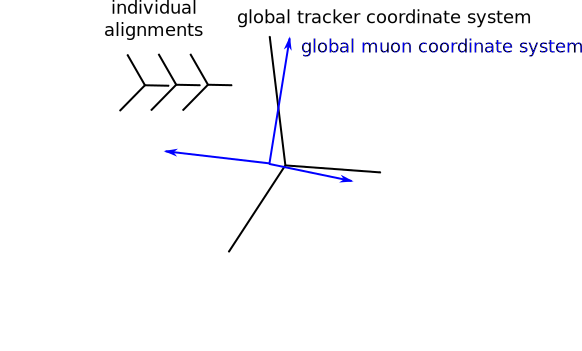
\includegraphics[width=\linewidth]{global_coordinate_systems.png}

\scriptsize
\begin{itemize}
\item Global coordinate system for (1) tracker, (2) muons, (3) ECAL, (4) HCAL
\item Separate database record, so global shifts/rotations can be
applied with more agility than individual alignment constants
\end{itemize}
\end{frame}

\begin{frame}
\frametitle{Conclusions}
\begin{itemize}\setlength{\itemsep}{0.4 cm}
\item While still working on full-scale procedure, we are focusing on
start-up
\item All HIP-related software is done (in 2\_0\_X) except monitoring plots
\item We're not waiting for MC: we can use existing samples
\item We can test beam-halo procedure in MTCC as soon as we're ready
\item With this timeline, we'll be ready for CRA0T/CRAFT data when
it becomes available
\item We'll also get as much information as we can from beam-halo
before first collisions
\end{itemize}
%% \hspace{-0.83 cm} \textcolor{darkblue}{\Large Outline2}
\label{numpages}
\end{frame}

\end{document}
